\chapter{Realtidsplanlægning}
\label{chap:rtp}
\fxnote{Kom ind på starvation et eller andet sted.}
Det andet anvendelsesområde vil vi behandle, med henblik på at inføre tid i \pycsp , er Real-time planlægning (RTP). Vi vil i dette kapitel gennemgå RTP samt diskutere hvordan det kan implementeres i \pycsp. 

RTP er baseret på den kendsgerning at nogle begivenheder i programmer kan være vigtigere at få udført end andre indenfor en afgrænset tidsperiode. Dette kan f.eks. være interrupts, input- eller output enheder eller interne processer. Med RTP tilknytter man en deadline for hver begivenhed, som bruges til at planlægge rækkefølgen for afvikling af begivenhederne. Formålet er at optimere antallet af begivenheder der når at blive udført inden deres deadline er overskredet. Normalt anses alle begivenheder for at være lige vigtige, og de planlægges ud fra en optimal udnyttelse af processoren. Denne optimale processorudnyttelse kan man være nødt til at gå på kompromis med hvis man ønsker at bruge RTP og derved prioritere visse begivenheder højere end andre. Man kan forestille sig en situation hvor man ikke starter en begivenhed med lav prioritet selv om den er klar, hvis man ved at en begivenhed med høj prioritet er klar kort tid efter, og venter derfor på at den er klar og igangsætter begivenheden med høj prioritet med det samme. 
RTP benyttes meget i specialiserede indlejrede systemer til f.eks medicinsk udstyr, kontrol af luftrummet, på rumstationen ISS\cite{Audsley1990} og mange andre steder. Det er dog også anvendeligt i mere gængse applikationer, typisk i forbindelse med en eller anden form for interaktion med den virkelige verden. 

I litteraturen omkring RTP bruges begreberne hard- og soft deadlines samt hard- og soft real-time systemer forskelligt, så vi vil i det følgende gennemgå hvordan vi definerer disse begreber. Vi har valgt at illustrere deadlines ved hjælp af time-value funktioner, hvor ``værdien'' indikerer det bidrag begivenheden bidrager med til systemets overordnede mål. 

\subsubsection{Kritisk deadline}
En kritisk deadline er en deadline som under alle omstændigheder skal overholdes for at opretholde systemets integritet. Såfremt en kritisk deadline overskrides vil der påføres skader på systemet som kan forårsage at systemets tilstand bliver udefineret. En kritisk deadline er illusteret på \cref{fig:hard-rtp}.

\begin{figure}
 \begin{center}
  \includegraphics[scale=0.75]{images/critical-deadline}
	\caption{Begivenhed med kritisk deadline.}
	\label{fig:hard-rtp}
\end{center}
\end{figure}


\subsubsection{Hard deadline}
Vi definerer en begivenhed til at have en hard deadline såfremt en færdiggørelse af begivenheden efter deadlinen ikke tilfører systemet nogen positiv værdi. Modsat en kritisk deadline kan en overskridelse af en hard deadline accepteres. På \cref{fig:hard-dl} vises en hard deadline for en begivenhed. 

\begin{figure}
 \begin{center}
  \includegraphics[scale=0.75]{images/hard-deadline}
	\caption{Begivenhed med hard deadline.}
	\label{fig:hard-dl}
\end{center}
\end{figure}

\subsubsection{Soft deadline}
Færdiggørelse af en begivenhed med en soft deadline, før dens deadline tilføjer den samme værdi til systemet som hvis den havde haft en hard deadline. Forskellen ligger i den tilførte værdi såfremt deadlinen overskrides. Hvor en hard deadline ikke tilføjer nogen værdi ved en overskridelse, vil en overskridelse af en soft deadline stadig tilføre en reduceret værdi ved færdiggørelse. Den tilførte værdi vil være omvendt proportional med længden af overskridelsen. \CRef{figure:soft-dl} illustrerer en soft deadline. 

\begin{figure}
 \begin{center}
  
\includegraphics[scale=0.75]{images/soft-deadline}
	\caption{Begivenheden med soft deadline.}
	\label{figure:soft-dl}
\end{center}
\end{figure}

\subsubsection{Hard real-time system}
Et hard real-time system er defineret ved et system der har begivenheder med hard deadlines, og kan garantere at disse ikke overskrides. Ydermere skal systemet være derterministisk, så denne garanti kan gives på forhånd. Det giver ikke mening at snakke om kritiske deadlines i hard realtime systemer da de kun adskiller sig fra hard deadlines med henblik på konsekvensen af en overskreden deadline, hvilket per definition ikke må ske i et hard real-time system.  

\subsubsection{Soft real-time system}
Et soft real-time system kan indeholde alle typer deadlines men opstiller ikke nogen garantier for at de overholdes. Det vil typisk bruge en algoritme til at op- og nedprioritere hvilke deadlines der skal overholdes såfremt alle deadlines ikke kan overholdes.

Generelt vil der i et real-time system ikke være alle begivenheder der har den samme type af deadline. Nogle begivenheder har ingen deadline, nogle har en soft deadline, og få har en hard eller eventuelt en kritisk deadline. 
 
\section{Planlægning af begivenheder}
Planlægningen af hvilke begivenheder der skal køres hvornår, tager udgangspunkt i det overordnede formål med systemet. Generelt vil formålet være at minimere antallet af overskredne deadlines, men dette er sjældent det eneste kriterie der planlægges efter. Ofte vil prioriteten for, og tiden det tager at udføre en begivenhed indgå i planlægningen. Eksempelvis vil man ofte prioritere at nå en kritisk deadline selv om det betyder at man overskrider to soft deadlines. 

%De fleste eksisterende real-time systemer arbejder på isolerede systemer, hvor planlæggeren har fuld kontrol over hele computeren. Derfor er hovedparten af forskningen indefor området gået til udarbejdelsen af specialiserede kerner og komplette operativsystemer\cite{damm1989real, jones1979staros, levi1989maruti,ramamritham14scheduling}. Vi ønsker i modsætning hertil ikke at udvikle en specialiseret kerne, men lade \sched en i \pycsp kunne planlægge processer efter bedste evne baseret på informationer den har om processerne.

For at foretage en planlægning af begivenheder der opfylder systemets formål bedst muligt, skal vi have så meget information om begivenheder som muligt - jo mere vi ved om dem jo bedre en planlægning kan der foretages. De relevante informationer i forhold til planlægningen er, hvornår en begivenhed forekommer, hvor lang tid den tager at udføre samt hvilken prioritet den har. 

Ud fra den tilgængelige viden kan der foretages en statisk eller dynamisk planlægning\cite{cheng1987scheduling}. Statisk RTP kræver at vi har alle de nævnte informationer om alle begivenheder. Herved kan vi på forhånd foretage en fuldstændig planlægning og allerede inden start have klarlagt om nogen deadlines vil blive overskredet. Såfremt vi ikke har alle informationer til rådighed, er vi nødsaget til at foretage en dynamisk planlægning. Dette vil ofte skyldes at vi enten ikke ved hvornår en begivenhed forekommer, eller at vi ikke har information om hvor lang tid der tager at udføre en begivenhed. \\
I praksis vil det være svært at opstille eksakte værdier for hvor længe en begivenhed er om at blive udført og der benyttes derfor ofte estimater i stedet for. \fxnote{hvilken betydning har det at der benyttes estimater i stedet for eksakte værdier?}

I systemer hvor begivenheder ikke er isolerede men kan have interne afhængigheder, kan der opstå det problem der hedder prioritetsinvertering\cite{sha1990priority}. Dette problem opstår hvis en begivenhed med høj prioritet er afhængig af en begivenhed med en lavere prioritet. Ikke nok med at begivenheden med høj prioritet må vente på den  begivenheden med lav prioritet. Den må også vente på alle begivenheder med medium prioritet. Derved bliver begivenheden i praksis kørt med den lavere prioritet da den ikke er klar før begivenheden med lav prioritet er færdig. Problemstillingen kan vises klart med følgende eksempel. Vi har tre begivenheder ($B_0,B_1,B_2$) med prioriteterne $Pr_0>Pr_1>Pr_2$. Først udvælges $B_0$ da denne har højst prioritet, men stopper da den er afhængig af kommunikation fra $B_2$. Den næste begivenhed der udvælges vil være $B_1$, og dermed bliver $B_0$ unødigt forsinket mens $B_1$ kører.

Overordnet set findes der to metoder til at minimere prioritetsinvertering. Enten kan man prøve at forhindre de opstår eller minimere/kontrollere prioritetsinverteringen. 
Hvis prioritetsinverteringen kommer som en konsekvens af brugen af kritiske regioner, kan man hindre processer i at blive afbrudt mens de er i de kritiske regioner. Dermed vil begivenheden med høj prioritet ikke skulle vente på begivenhederne med medium prioritet, men omvendt skal den altid vente på processen med lav prioritet, selvom den ikke ønsker at tilgå den kritiske region. 

Er begivenhederne alle regelmæssige og det er kendt hvor lang tid hver begivenheden tager, kan man nægte at lade begivenheder tilgå kritiske regioner, hvis der er mulighed for de så blokere for begivenheder med højere prioritet.

Prioritetsnedarvning er en tredje metode til at kontrollere prioritetsinvertering\cite{sha1990priority}. Ved at benytte denne løsning vil en begivenhed med lav prioritet, som en begivenhed med høj prioritet er afhængig af, nedarve prioriteten fra den begivenhed der venter på den. Herved sikres det at begivenheder med høj prioritet ikke kommer til at vente unødigt på begivenheder med lav prioritet. 

%Overordnet kan begivenheder planlægges enten statisk eller dynamisk\cite{cheng1987scheduling}. I statisk RTP er alle begivenheder kendt på forhånd. Planlæggeren kan i dette tilfælde allerede inden start udregne om det er muligt at overholde alle deadlines. Alternativt planlægges begivenhederne dynamisk hvis der uregelmæssigt kan ankomme nye begivenheder der skal planlægges. 

%\fxnote{Motivationen her skal være at vi skal kende begivenheders frekvens og længde - skriv noget om det!}
%I realtidssystemer er næsten alle begivenheder cykliske, med enten en regelmæssig eller tilfældig frekvens. Begivenheder der forekommer med en regelmæssig frekevens kan være f.eks. være målinger der skal foretages med bestemte intervaller, hvor uregelmæssig frekvens ofte vil være tilfældet ved begivenheder der skal indtræffe som reaktion på udefrakommende input, f.eks. fejl eller alarmer. 

%\begin{shaded}
%Til planlægningen har planlæggeren behov for at vide hvor lang tid det vil tage at udføre en given begivenhed per periode, men da dette tal enten ikke er kendt eller fast for hver periode, bruges der ofte estimater. Dette medfører at en aperiodisk begivenhed kan ankomme på et vilkårligt tidspunkt og da planlæggeren kun har et estimat for tidsforbruget kan man  ikke tilknytte en ``hard deadline'' til aperiodiske begivenheder, da der altid findes en kæde af aperiodiske begivenheder der medfører en overskridelse af en deadline. 
%\end{shaded}

%\fxnote*{Dette skal måske flyttes eller omformuleres så vi ikke med det samme begrænses til dynamiske \sched}{I \pycsp kan der til alle tidspunkter tilføjes nye processer, og derfor vil vi kun beskæftige os med en dynamisk \sched. Desuden har man ikke med \pycsp fuld kontrol over hele operativsystemet. Mængden af processerkraft vi har til rådighed til kørsel af processerne vil derfor varriere uafhængigt af \pycsp, hvorfor vi heller ikke kan lave et pålidelig ``hard real-time system'', men fokusere på et ``soft real-time system''.}

\subsection{Metoder til skemaplanlægning}
Der findes adskillige metoder til at planlægge rækkefølgen af begivenheder. De adskiller sig fra hinanden med henblik på hvilke informationer de benytter og hvad de optimerer efter. Vi har valgt at kigge på ``Rate monotonic algorithm''\cite{lehoczky1989rate,liu1973scheduling} og ``Earliest deadline first''\cite{liu1973scheduling} indenfor henholdsvis statisk og dynamisk skemaplanlægning.

Hvor begivenheder isoleret set har behov for at udføre deres opgave inden deres deadline, har \sched en behov at foretage en kvantitativ vurdering af en proces' prioritet og organisere dem så den, til enhver tid, kan vælge hvilken proces, der skal udføres som den næste. Hovedformålet for en  \sched ~ er derfor at gå fra en række processer med tilknyttet deadline og eventuelt andre egenskaber til en prioriteret liste. 

Der fokuseres i litteraturen på om en algoritme er stabil eller ej. Såfremt en algoritme er stabil vil man kunne definere en delmægnde af begivenheder, for hvilke man kan garantere at de ikke overskrider deres deadline. 

\subsubsection{Rate monotonic algorithm (RM)}
RM er en statisk \sched, der fra start af udregner en prioriteret liste på baggrund af frekvensen af processens periode, dermed vil processer der ofte skal have udført deres periode få en højere prioritet end processer med lav frekvens. RM er todelt og i første del udføres før selve simuleringen udregnes  prioriteten for processerne, og udvælger hvilke processer der kan medtages i selve udførslen. Anden del står for udvælgelsen af processer  under simuleringen, og her vælges simpelt den proces med den højeste prioritet. 

Et problem for RM er at ved udvælgelsen af processer der kan medtages har man ikke en optimal udnyttelsen af processorkraft. \Citeauthor{lehoczky1989rate} er kommet frem til at ``worst-case'' er udnyttelsen i gennemsnit 69\% \cite{lehoczky1989rate}. Et større problem i relation til implementering i \pycsp er dog at RM er dog at den er statisk. Til gengæld er algoritmen stabil ved en overskridelse af deadline for en proces. 

\subsubsection{Earliest deadline first (EDF)}
Som alternativ til den statiske \sched, hvor man ikke kan ændre prioriten af processen løbende under udførslen, findes de dynamiske \sched er, hvor er EDF er et eksempel. Her evalueres prioriterne af processerne dynamisk under udførslen og evaluerer dermed løbende hvilke processer der skal udvælges. I EDF har den proces hvis deadline ligger først højest prioritet og den proces hvis deadline ligger længt ude i fremtiden har lavest prioritet. I EDF er antallet af prioriteter ikke fastlagt på forhånd og antallet, samt spændet mellem højeste og laveste prioritet, kan ændre sig dynamisk. Aperiodiske processer kan i EDF indgå på lige fod med de periodiske da man til hvert processkift evaluere hvilken der har den nærmeste deadline, som både kan være en periodisk proces som en aperiodisk.

Udnyttelsen af processorkraft kan i EDF komme op på 100\%, da alle processer bliver planlagt løbende i modsætning til RM der foretager et valg om en given proces kan planlægges.  Ulempen ved EDF er den ikke er stabil idet vi ikke har kontrol over hvilke processers deadline der bliver overskredet. Dette er specielt et problem hvis man har en en uhomogen samling processer hvor en mindre del er kritiske. Såfremt skemaplanlæggeren ikke kan foretage preemptive skift mellem begivenheder kan EDF ikke give nogen garanti om at alle deadlines overholdes, selv om der findes en rækkefølge af begivenheder der sikrer dette. Dette er illustreret på \cref{fig:edf-nonpreemptive}.

\begin{figure}
 \begin{center}
  \includegraphics[scale=1.00]{images/edf-nonpreemptive}
  \caption{Overskridelse af deadline med EDF såfremt der ikke kan udføres preemptive kontekstskift. Begivenheden $B_2$ ankommer til tiden $t_1$ og har deadline ved $t_5$. Den kan dog ikke igangsættes før $B_1$ er færdig, hvorved $B_2$ overskrider sin deadline. Figuren er kopieret fra \cite[56]{buttazzo2005}}
  \label{fig:edf-nonpreemptive}
  \end{center}
\end{figure}

\subsubsection{Least Laxity(LL)}
LL er en modifikation af EDF. LL kigger på hvor lang tid en begivenhed tager at udføre sammenholdt med hvor lang tid der er til deadline for begivenheden. Laxity er defineret som deadline minus tiden det tager at udføre begivenheden. Laxity bliver altså et udtryk for hvor presserende det er at igangsætte en begivenhed for at den kan nå sin deadline. I LL bruges dette til at prioritere de begivenheder der har mindst laxity højest når begivenhederne planlægges. 

\section{Realtime planlægning i \pycsp}
\label{sec:rtp-pycsp}
\fxwarning{Skriv afsnit om udvælgelse af kanal efter prioritet}

Da vi ønsker at introducere RTP i \pycsp er der er række forhold som vi skal tage højde for. Vi vil i dette afsnit tage udgangspunkt i de ovenstående opstillede muligheder og sammenholde dem med \pycsp. 

I \pycsp kan vi anskue processerne som begivenheder, og derved bruge skemaplanlæggeren i greenlets-versionen til at styre hvilken proces og dermed hvilken begivenhed der udføres. Vi har ikke umiddelbart informationer om hvor lang tid en proces er om at blive udført, og det vil kræve en analyse af den enkelte proces at udlede estimater for det. Vi har valgt at fokusere på selve planlægningen af processerne og ikke analyse af processerne. Dermed har vi ikke mulighed for både at benytte RM og LL algoritmerne da de begge benytter information om udførselstiden for en proces. Derved har vi EDF tilbage som mulighed, hvilket er den algoritme som vi vil implementere. En udviddelse af \pycsp til at benytte EDF er forholdsvis ligetil. Der skal laves en mulighed for at brugeren kan angive en deadline til en proces, og vi skal ved kontekstskift sikre at vi aktiverer den proces der har den førstkomne deadline. \pycsp har per definition interne afhængigheder mellem processerne i form af kommunikation over kanaler, og vi kan derfor opleve problemer med prioritetsinvertering. Vi skal derfor også implementere prioritetsnedarvning for at sikre os mod prioritetsinvertering. Endeligt skal vi håndtere overskredne deadlines.

Da vi benytter os af greenlets-versionen af \pycsp arbejder vi med en skemaplanlægger der ikke kan foretage preemptive kontekstskift. Dette kan lede til problemstillinger som det illustreret på \cref{fig:edf-nonpreemptive}. En metode til at mindske denne type problemer er at lade de enkelte processer afgive kontrollen med jævne melemrum. Herved vil der blive foretaget en ny evaluering om hvilken proces der skal aktiveres, og hvis der processer der har en nærmere deadline som er blevet klar, aktiveres en af disse. Dette beror helt og holdent på hver at hver enkelt proces frivilligt afgiver kontrollen og gør det med jævne mellemrum når den er aktiv. Dette betyder at det er overladt til udvikleren at indsætte det på relevante steder i processens kode. 



% Nedenstående beskrives i implementationen
%Vi har valgt at abstrahere en deadline til en prioritet, da vi hermed åbner for senere at kunne lade andre faktorer indgå i prioriteten end blot en proces' deadline. 

begrænset forhåndsviden 
  dynamisk planlægning
  ingen viden om udførselstid - heller ikke estimater  

non-preemptive (snakkes der ikke om i foregående afsnit)

nedarvning
  any->any kanaler kan potentielt give stor spredning af prioritet

\subsection{Prioritetsnedarvning}
At introducere prioritetsnedarvning i \pycsp virker umiddelbart ligetil idet vi kan se de indbyrdes afhængigheder klart ud fra forbindelserne gennem kanaler. Der kan forekomme andre afhængigheder som er mindre synlige, men vi mener ikke disse vil forekomme i velskrevne CSP applikationer, og vi har derfor valgt at begrænse os til afhængigheder repræsenteret vha. kanaler. På trods af den umiddelbare simplicitet er der dog adskillige overvejelser bl.a. med henblik på hvilke konstruktioner i \pycsp der skal arve prioriteter, hvornår de skal arve dem og hvor længe de skal beholde den modificerede prioritet. \\

\subsubsection*{Ændring af prioritet}
Det er væsentligt at overveje hvornår det er nødvendigt at foretage prioritetsnedarvning. Vi arbejder med et dynamisk system af processer, hvor en proces, afhængig af dens tilstand, er afhængig af forskellige andre processer for at kunne arbejde videre. Hvis vi højner prioriteten på alle processer der er forbundet til en proces med høj prioritet vil mange af processerne der arver den høje prioritet reelt ikke kunne bidrage til udførelsen af den proces der starter med høj prioritet. Det er en bedre løsning at det kun er den eller de processer der kan sikre videre udførsel af den aktuelle proces der tildeles højere prioritet. Hvis eksempelvis en proces med høj prioritet ønsker at skrive på en kanal, skal alle processer der læser på den kanal arve den høje prioritet, men processer som ønsker at skrive til en anden kanal som processen med høj prioritet læser fra, skal ikke arve den høje prioritet. Dette vil selvfølgelig ændre sig lige så snart processen har fået skrevet på kanalen og derefter befinder sig i en anden tilstand og er afhængig af noget andet for at komme videre i sin udførsel. \\
Ud fra dette kan vi også se at så snart, det midlertidige afhængighedsforhold ophører skal processer der har arvet en prioritet miste denne. Der skal selvfølgelig tages højde for at en proces kan arve forskellige prioriteter fra forskellige andre processer, så det skal være muligt at falde tilbage til den næsthøjeste arvede prioritet, i stedet for blot at skifte tilbage til den oprindelige prioritet. 

\subsubsection*{Begrænsning af nedarvning}
Vi har som nævnt en klar kæde af afhængigheder i \pycsp men vi skal være opmærksomme på ikke at højne processers prioritet unødigt. Dette kan let være tilfældet såfremt vi ikke holder ordentligt styr på hvorfor en proces har den prioritet den har, om den er sat af udvikleren eller den er nedarvet. Man kan forestille sig en situation hvor et uddrag af et proces-neværk består af en generator-forbruger model med to generatorer og en enkelt forbruger. De to generatorer er forbundet til forbrugeren vha. en \code{alternation} og generatorerne har henholdsvis høj og lav prioritet. Forbrugeren vil i dette scenarie arve den høje prioritet fra den tilsvarende generator, men utilsigtet vil den høje prioritet også propagere fra forbrugeren til generatoren med lav prioritet. Dette er ikke hensigtsmæssigt da de to generatorer nu har lige høj prioritet og ikke det forhold som udvikleren oprindeligt har angivet. Dette problem kan løses ved at indføre en enkelt restriktion af prioritetsnedarvning, hvilket er ensretning af nedarvningen med henblik på om der skal læses eller skrives til en kanal. Det vil sige at en proces der arver en høj prioritet fordi den skal læse fra en proces med højere prioritet, som i førnævnte generator-forbruger model, kun propagerer den høje prioritet videre til processer som den skal skrive til. Derved udgår vi den uhensigtsmæssige tilbageførelse af prioritet samtidig med at vi bibeholder nedarvning frem i systemet.

\subsubsection{noter}
Skelne mellem read og write
måske skal en kanal arve prioritet?
hvornår skal prioriteten ændres? 

2 cases:
udvælgelse i alternation
propagering af prioritet

med nedarvning kan en proces uden deadline arve en høj prioritet uden at få sat en deadline. 

Skal processer der arver prioritet også arve deadline? Det skal de nok ikke, da de så kommer til at kaste exceptions selv på deadlines som brugeren ikke har sat. De skal nok kastes af den oprindelige proces med information om hvad den ventede på da den fejlede. 

\subsection{Tilknytning og overskridelse af deadlines}
Som udgangspunkt skal vi kunne håndtere at en proces kan have forskellige typer deadlines. Umiddelbart giver det mening at der for hver proces tilknyttes en deadline samt hvilken type det er. Dette giver mulighed for at vi kan differentiere i måden hvorpå vi håndterer en overskreden deadline. F.eks. kan vi stoppe systemet helt i tilfælde af overskridelse af en kritisk deadline, kaste en exception ved en hard deadline og blot registrere overskridelser af soft deadlines. Uanset hvilken handling vi vælger at tilknytte til de respektive overskridelser, vil der være situationer hvor den vlagte handling ikke er optimal. Vi har derfor valgt en anden løsning hvor en proces blot kaster en exception hvis den overskrider en deadline. Dette overflødiggør at der tilknyttes en specifik type deadline til en proces, da håndteringen af den kastede exception overgives til udvikleren. Det er herved op til den nekelte udvikler at definere hvad der skal ske i i hver enkelt proces såfremt den oplever en overskreden deadline. Dette giver den største frihed til at tilpasse håndteringen til den enkelte proces og applikation. 

\begin{shaded}
\subsection{Blokkerede processer}
I den teoretiske tilgang til RTP antages det ofte at processerne er periodiske, har en fast eksekverings tid per periode og er uafhængig af andre processer, og køres i et isoleret miljø. De forskellige tilgange til RTP fokuserer på hvordan man kan overvinde de enkelte antagelser ved isoleret og ophæve en af begrænsningerne. 


Dette er en højst idealiseret verden og i en introduktion af RTP i PyCSP vil processerne ikke overholde et eneste af disse antagelser. 
I \pycsp bruges rendezvous til at blokere kommunikerende processer.

Vi vil nu beskrive problemerne ved at processerne er afhængige af hinanden, og kan blokere hinanden, således at en proces med høj prioritet venter på processer med lavere prioritet. Forestil dig i \pycsp tre processer ($P_0,P_1,P_2$)med prioriteterne $Pr_0>Pr_1>Pr_2$. Først udvælges $P_0$ da denne har højst prioritet, men stopper da den skal kommunikere med $P_2$. Den næste proces der udvælges vil være $P_1$, og dermed bliver $P_0$ unødigt forsinket mens $P_1$ kører. Dette kaldes priority inversion\cite{sha1990priority}.

Der findes overordnet set to metoder til at løse problemet med priority inversion. Enten kan man ungå at blokere processer, eller man kan benytte priority inherience\cite{sha1990priority}. Med \pycsp kan man ikke ungå at processer kommunikere, og dermed vil kunne blokere hvorfor priority inherience er den enste farbare vej hvis man skal sikre optimal planlægning.
\end{shaded}



\section{Slagterieksempel}
\fxnote{mere intro}
I det første eksempel på en applikation der kan bruge et RTP systemer, skal vi udvikle er en beslutningsmodel, der kan beslutte hvilken model robotten skal bruge til at  udskære den enkelte gris med. På Danish Crown slagteriet i Horsens udskæres grisene af en robot som beskrevet på deres hjemmeside:

\begin{quote}\textit{``Grisen [\ldots] skal nu skæres i mindre, håndterbare stykker. Det sker i en meget avanceret maskine -- en såkaldt tredeler -- hvor hver halvdel af grisen deles i tre stykker: bov, mellemstykke og skinke. \\ 
\\
Robotten starter med at fotografere hver halvdel. Dataene fra billedet kombineres med ordren og kundens ønsker, hvorefter stykket deles i tre - nøjagtigt afpasset kundens ønsker.''}{ Danish Crowns hjemmeside\footnote{\url{http://www.danishcrown.dk/custom/horsens/3772.asp}}}\end{quote}

Et billede af den automatiske tredeler er vist  på \cref{fig:pig}. Vi forestiller os at selve udskæring også laves på baggrund af en model af hvordan grisen er udformet. Det har dog vist sig at modellen ikke altid resulterer i en  optimal udskæring, da  ca. 10\% af alle grise har et ekstra sæt ribben som modellen ikke tager højde for. Til at løse dette problem har slagteriet udviklet en ny model for grise med et ekstra sæt ribben.

\begin{figure}
 \begin{center}
  \includegraphics[scale=0.5]{images/209690-1}
	\caption{Billedet viser i forgrunden  et foto taget af tredeleren til brug for analyse. I baggrunden ses transportbåndet, hvor de halve  grise venter på på at blive udskåret af den automatisk tredeler.}
	\label{fig:pig}
\end{center}
\end{figure}


Slagteriet har placeret kameraet i starten af et transportbåndet mens udskæringsrobotten findes i den anden enden. Der kan være flere svin på transportbåndet på samme tid, og det fremføre svinene i et fast tempo. Dette giver et fast tidsrum fra svinet passere kameraet til det passere robotten. Vi har hermed et klassisk RTP system, hvor robotten skal foretage et valg af model under en hard deadline, da det ikke er en mulighed ikke at foretage en udskæring.

Vi må først se på arbejdsgangen der er involveret i valget af model. 
\begin{enumerate}
\tightlist
	\item Et billede bliver taget af svinet mens den passere kameraet.
	\item Billedet konverteres til en 3D-model af svinet.
	\item 3D-modellen analyseres.
	\item Modellen udvælges på baggrund af analysen, ordren og kundens ønske.
	\item Robotten udskærer grisen.
\end{enumerate}

Man kan se at arbejdsgangen indeholder en  række klart afgrænsede arbejdsområder, som med fordel kan modelleres som selvstændige processer i \pycsp. Der findes do ikke kun en måde at opbygge procesnetværket på, men vi har valgt at have følgende processer: Røntgenskanner, Billedekonvertering, 3D-analyse og en udvælgelse og udskæringsproces, hvilket leder til et procesnetværk som vist i \cref{fig:pig-network}.

\begin{figure}
 \begin{center}
  
\includegraphics[scale=1]{images/pig-network}
	\caption{Procesnetværk til udskæring af svin på et slagteri.}
	\label{fig:pig-network}
\end{center}
\end{figure}



\subsubsection*{Implementering i Greenletsversionen}
Til at implementere eksemplet uden brug af af RTP-udvidelsen i \pycsp, kan vi oprette hvert svin som et objekt og tilknytte en deadline. Nu kan hver proces evaluere om svinet har overskredet sin deadline, i det tilfælde fjerne svinet, og stoppe den videre behandling. Det er ikke angivet hvordan hele processen startes, men vi antager der findes en form for detektor foran røngtenkameraet, der opfanger når et svin passere og som dermed  starter processen. 
Når detektoren starter hele processen, opretter den svineobjektet som den sender til Røngtenprocessen, samt sender en kopi direkte til udvælgelse og udskæringsprocessen. dermed ved processen at der ankommer et svin som den skal udskære, og hvis den inden deadline får en analyse af svinet, kan den træffe et begrundet valg om hvilken model der skal bruges,  men hvis ikke denne analyse findes, bruges blot standardmodellen. \CRef{fig:pig-network2} viser det endelige  netværk, hvor detektoren er introduceret, og som sender data til hhv. Røntgenprocessen og til Udvælgelse og udskæringsprocessen. 

\begin{figure}
 \begin{center}
  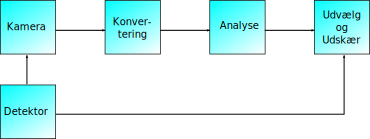
\includegraphics[scale=1]{images/pig-network2}
	\caption{Procesnetværk med detektor til initiering af hvert svin.}
	\label{fig:pig-network2}
\end{center}
\end{figure}

Et problem ved at implementere hele slagterieksemplet i \pycsp er  grænsefladen mellem verden hvor grisene kører på transportbåndet, og  greenletsversionen,  hvor  kun en proces kan være aktiv af gangen. Konvertering og analyse processen arbejder, mens  udskæringsprocessen venter på at svinene kommer inden for rækkevidde. Konvertering- og analysenprocessen  skal dog frivilligt afgive kontrollen, mens svinet er indenfor robottens rækkevidden og hvis de ikke gør, bliver svinet ikke udskåret. I stedet for at det samme system både skal foretage analysen som  styrer robotten, kan vi antage at processerne er mere autonome i deres opbygning. Dette giver at computeren der styrer robotten fungere uafhængigt af de computere der foretager konvertering og analysen. de to computere kan udveksle data igennem f.eks en database, harddisk eller anden delt datastruktur. Hvis analysen bliver færdig gemmes den, i den delte datastruktur, og robotten kan udnytte analysen, Hvis ikke den er klar bruges standard modellen.    



%\subsection{Eksempel 2 - Sensornetværk med høj/lav -prioritet}
%\inline{eks2: skal vise alternation, kan være en sensor som modtager måledata med lav prioritet og som skal sende måledata på opdordring med høj prioritet.}

\section{Implementering}

\begin{itemize}
\item DeadlineException
\item Now
\item Release() f.eks i iterationer
\item to køer kaldet has\_priority og no\_priority, og deres brug i funktionen activate
\item Process udvidet med: \\self.inherit\_priotity = []     \\
        self.deadline = None\\
        self.internal\_priority = float("inf")\\
        self.has\_priority = False\\
            if isinstance(arg, pycsp.greenlets.channelend.ChannelEndRead):\\
                arg.channel.\_addReaderProcess(self)\\
            if isinstance(arg, pycsp.greenlets.channelend.ChannelEndWrite):\\
                arg.channel.\_addWriterProcess(self)
\item def Set\_deadline(value,process=None):
\item def Remove\_deadline(process=None):
\item def SetInheritance(process):
\item def ResetInheritance(process):
\item Channel:\\
        self.readerprocesses = []\\
        self.writerprocesses = []

\item Udviddet _read og _write
\item Udvidder match


\end{itemize}

\section{Evaluering}
  \inline{Evaluering af hvordan eksemplet løses efter den valgte 
  implementering benyttes. Inkluderer test+performance}
\subsection{Test af korrekthed}
  Vi har igennem designet og udviklingen af \code{simulerings}-versionen brugt en Test Driven Development (TDD). I TDD starter man med at skrive tests til en ny egenskab der skal udvikles. Designet er implementeret korrekt når testene kan gennemføres korrekt. Dette medfører at vi løbende i forbindelsen med udviklingen af \emph{simulerings}-versionen har skrevet tests. Desuden har vi integreret alle tests fra \emph{greenlets}-versionen ind i \emph{simulerings}-versionen, således at tests skrevet til \emph{greenlets}-versionen også tester vores version. Resultaterne af testene kan ses i tabel \fxerror{TODO! testene virker ikke:(}
  
\subsection{Eksempler}



\subsection{Effektivitet}  
\inline{skal vi overhoved evaluere performance?}
  


\section{Fremtidigt arbejde}\label{sec:deadlineFuture}
Vi har i dette kapitel opstillet en basal model for en RTP-implementering i \pycsp. Implementeringen er foretaget med henblik på blot at vise muligheden for en sådan model, og der er flere udviddelser som vi mener vil kunne forbedre modellen såfremt de kan implementeres. Vi vil i dette afsnit gennemgå nogle forbedringer som vi mener er interessante, men som ikke er inddraget i den basale implementering. 

\subsubsection{Evaluering af effektivitet}
Vi har med eksempler og test vist, at den implementerede løsning fungerer teoretisk korrekt. Vi har ingen test af om vi reelt når flere deadlines med vores RTP-løsning end vi ville uden. Vi har ikke nogle reelle tal for hvor meget tid vi bruger på at evaluere hvilken proces der skal aktiveres, samt opretholde de metadata der skal til for at foretage denne vurdering. En grundig analyse af tidsforbruget i de administrative dele af vores implementering ville derfor være interessant at udføre, så man bl.a. kan udlede generelle retningslinier for hvor ofte det vurderes hvilken proces der skal køre og hvor beregningstung hver proces bør være for at opnå den bedste ydelse. 

\subsubsection{Estimater for udførselstid}
Den primære begrænsning i vores løsning er manglen på at kunne evaluere hvor lang tid en proces eller dele af en proces tager at udføre. Hvis vi kunne udvikle en løsning der kunne foretage estimater af processers udførselstid ville vi kunne vælge en anden udvælgelsesalgoritme, som f.eks LL frem for EDF. Derved ville udvælgelsen af hvilken proces der skal aktiveres blive mere præcis. Ligeledes vil muligheden for at vurdere hvor langt en proces er nået i sin udførsel også være meget brugbart i forbindelse med prioritetsnedarvning. I vores implementering nedarver vi prioritet til alle processer som har mulighed for at opfylde en afhængighed. Såfremt vi kan vurdere hvilken proces der er tættest på at kunne opfylde afhængigheden, kan vi nøjes med at nedarve prioriteten til denne proces. Dette vil afhjælpe problemet med prioritetsdevaluering som nævnt i \cref{sec:aendring-af-prioritet}.

\subsubsection{Håndtering af forskellige typer deadlines}
I den nuværende løsning håndterer vi alle deadlines ens. Det er der fordele og ulemper ved, hvor en fordel er, at udvikleren får maksimal kontrol over hvad der skal ske såfremt en given deadline overskrides. Vi håndterer overskridelser af deadlines ved at kaste en exception når det sker. Dette er måske ikke altid ønskværdigt hvis det er en soft deadline der overskrides, da processen derved afbrydes. Det kunne tænkes at der er tilfælde hvor det er mere hensigtsmæssigt at udføre processen helt, og først her give besked om at den ikke nåede sin deadline.

\subsubsection{Udviklerbestemte prioriteter}
På nuværende tidspunkt har alle processerne den samme prioritet inden de planlægges, og deres prioritet afhænger udelukkende af deres deadline. Det kunne være interessant at undersøge om man kan bruge en anden \sched, der kan håndtere at processerne har forskellige prioriteter inden de blev planlagt.

Hvis muligheden  for at differentiere processerne blev implementeret, kunne det være spændene hvis man kunne udvide \sched, så udvikleren kunne angive et kritisk sæt af processer, for hvilke det kunne garanteres at de ikke ville overskrider deres deadline. 

%\subsubsection{Implementering i andre \pycsp versioner}
%Det kunne være interessant at undersøge mulighederne for for at lave en implementering af RTP i andre versioner af \pycsp. Dette vil åbne op for de muligheder der er tilknyttet de forskellige implementeringer, hvilket vil gøre RTP mere praktisk anvendelig. Specielt er muligheden for brug af flere processorer med enten threads\footnote{Ved brug af eksterne moduler}- eller process-versionen. Dette vil dog, som tidligere nævnt, kræve at skemaplanlægningen flyttes til operativsystems skemaplanlægger og bliver derved 


%Test af effektivitet

%Estimater for kørselstid for processer

%Evaluering af hvor langt en proces er fra at være færdig

%Implemementering i process-version

%\begingroup
%\setsecnumdepth{part} 
\chapter{Konklusion} 
\label{chap:konklusion}

Vores mål med dette speciale var, at undersøge muligheden for, at lave en udvidelse af \pycsp, der muliggør brugen af tid direkte i sproget. Der findes allerede et massivt teoretisk arbejde indenfor området, men ingen praktisk anvendelige implementeringer, så vores fokus har været på, at det skulle være praktisk anvendeligt. Dette afspejles ved, at vi har valgt at benytte eksempler som omdrejningspunkt for vores analyser af de tre anvendelsesområder. 

De tre anvendelsesområder vi identificerede i introduktionen var diskret simulering, realtids-planlægning og interaktiv tid. Vi har gennem vores analyse kommet frem til at det er mere hensigtsmæssigt at anskue anvendelsesområderne ud fra hvilken tidsmodel de bygger på. \CRef{fig:timemodel} viser således opdelingen af anvendelsesområderne i henholdsvis diskret og realtid.

\begin{figure}[htp]
 \begin{center}
  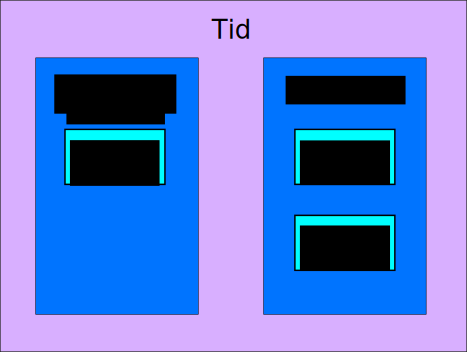
\includegraphics[scale=0.6]{images/timemodel}
	\caption{Forholdet mellem de tre anvendelsesområder af tid vi opstillede i introduktionen.}
	\label{fig:timemodel}
\end{center}
\end{figure}

Indenfor diskret simulering har vi udviklet en løsning, der er let at anvende, og som eliminerer kravet om en delt datastruktur for at administrere tid i \pycsp. Yderligere kræver løsningen væsentligt mindre kode til at administrere tiden, end en tilsvarende løsning lavet i ren \pycsp. 
Sammenligner vi vores løsning med \simpy, der er et framework til simuleringer, skrevet i Python, mener vi at vores løsning er mere intuitiv og fleksibel at benytte, til at modellere et givet problem. Dette tillægges i høj grad at vi direkte kan benytte \pycsp's processer og kanaler. Et eksempel på hvordan diskret simulering i \pycsp giver udvikleren større frihed til sin modellering finder vi i en kommende udvidelser til \simpy. De arbejder  på at udvide deres framework til at kunne håndtere reservation af flere begrænsede ressourser som skal benyttes samtidigt. Dette er allerede muligt i vores løsning, uden det har været vores fokus, da ressourcer blot modelleres som processer i \pycsp. Ønsker man at reservere flere ressourcer, kommunikerer man blot med flere processer, og når alle processerne har svaret, holder man alle de begrænsede resourcer. Arbejdet kan nu udføres, og ressourcerne frigives igen. 

I vores løsning til realtidsplanlægning har vi implementeret EDF, som den grundlæggende algoritme til at bestemme rækkefølgen, for udførsel af processer. Vi har implementeret prioritetsnedarvning for at imødekomme problemer med prioritetsinvertering, samt indført en prioriteret udvælgelse i \code{alternations} og når der kommunikeres over kanaler. Vores eksempel viser tydeligt at vores RTP-løsning kan gøre en forskel, såfremt der i programmet, kan foretages en differentiering i prioriteten af de processer der skal afvikles. 

Vi er kommet frem til at interaktiv planlægning ikke kan anses som et selvstændigt anvendelsesområde, men nærmere som en gren af realtidsplanlægning. De benytte begge realtid som tidsmodel, og har deadlines og prioriteter. Interaktiv planlægning har yderligere tilføjet et starttidspunkt, men det ændrer ikke fundamentalt på modellen. 

Vores løsninger er brugbare i den nuværende form, men der kan foretages en række udvidelser der vil gøre dem endnu mere anvendelige. 
Indenfor \des synes vi det kunne være spændende at udvide løsningen til at kunne foretage en dynamisk evaluering af køer, for derved at give ekstra fleksibilitet i de udviklede simuleringer. I RTP har vi lavet en basisimplementation der benytter EDF. Det kunne være interessant at kigge på mulighederne for at bedømme en proces' udførselstid, eller lade udvikleren angive dette. Det vil åbne op for brug af andre algoritmer end EDF, hvorved der åbnes op for brug af adskillige andre algoritmer til skemaplanlægningen og udvider anvendelsesområdet.  

%lettere at modellere processer
%Simpy kan ikke reservere begrænsede ressourcer

%Sammenligning med Simpy her 

%Tidsmodeller/anvendelsesområder

%Praktisk anvendelig implementering

%nuværende tilstand for anvendelsesområderne

%\endgroup 


